\gaokaoheader{2020}{海南卷}





\gaokaoxz


\begin{enumerate}
	%\renewcommand{\labelenumi}{\arabic{enumi}.}
	% A(\Alph) a(\alph) I(\Roman) i(\roman) 1(\arabic)
	%设定全局标号series=example	%引用全局变量resume=example
	%[topsep=-0.3em,parsep=-0.3em,itemsep=-0.3em,partopsep=-0.3em]
	%可使用leftmargin调整列表环境左边的空白长度 [leftmargin=0em]
	\item
	$ 100 $年前,卢瑟福猜想在原子核内除质子外还存在着另一种粒子$ X $,后来科学家用$ \alpha $粒子轰击铍核证实了这一猜想,该核反应方程为:${ }_{2}^{4} He+{ }_{4}^{9} Be \rightarrow{ }_{6}^{12} C+{ }_{n}^{m} X$,则 \xzanswer{A}

 

\fourchoices
{$m=1, \quad n=0, \quad X$ 是中子}
{$m=1, \quad n=0, \quad X$ 是电子}
{$m=0, \quad n=1, \quad X$ 是中子}
{$m=0, \quad n=1, \quad X$ 是电子}



\item
如图,上网课时小明把手机放在斜面上,手机处于静止状态。则斜面对手机的 \xzanswer{B} 
% TODO: \usepackage{graphicx} required
\begin{figure}[h!]
	\centering
	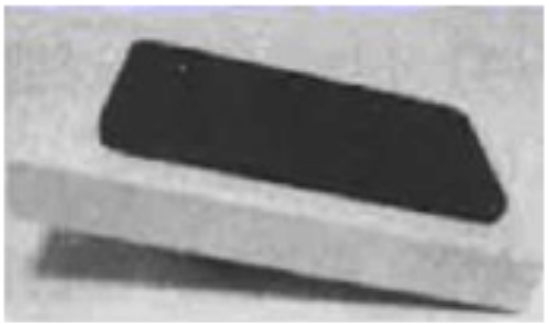
\includegraphics[width=0.18\linewidth]{picture/screenshot092}
\end{figure}

\fourchoices
{支持力竖直向上}
{支持力小于手机所受的重力}
{摩擦力沿斜面向下}
{摩擦力大于手机所受的重力沿斜面向下的分力}



\item
图 \subref{2020海南3a} 、 \subref{2020海南3b} 分别表示两种电流的波形,其中图 \subref{2020海南3b} 所示电流按正弦规律变化,分别用$ I_{1} $和$ I_{2} $表示 \subref{2020海南3a} 和 \subref{2020海南3b} 两电流的有效值,则 \xzanswer{D} 
\begin{figure}[h!]
	\centering
	\begin{subfigure}{0.4\linewidth}
		\centering
		\includesvg[width=0.6\linewidth]{picture/svg/GZ-3-tiyou-1687} 
		\caption{}\label{2020海南3a}
	\end{subfigure}
	\begin{subfigure}{0.4\linewidth}
		\centering
		\includesvg[width=0.6\linewidth]{picture/svg/GZ-3-tiyou-1688} 
		\caption{}\label{2020海南3b}
	\end{subfigure}
\end{figure}


\fourchoices
{$I_{1}: I_{2}=2: 1$}
{$I_{1}: I_{2}=1: 2$}
{$I_{1}: I_{2}=1: \sqrt{2}$}
{$I_{1}: I_{2}=\sqrt{2}: 1$}





\item
 一车载加热器(额定电压为 $24 \ V$ )发热部分的电路如图所示, $a$ 、$ b $、$ c $ 是三个接线
端点, 设$ ab $、$ ac $、$ bc $ 间的功率分别为 $P_{ab} $、$ P_{ac} $、$ P_{bc} $, 则 \xzanswer{D} 
\begin{figure}[h!]
	\centering
	\includesvg[width=0.23\linewidth]{picture/svg/GZ-3-tiyou-1689}
\end{figure}


\fourchoices
{$P_{ab}>P_{bc}$}
{$ P_{a b}=P_{a c}$}
{$P_{ac}=P_{b c}$}
{$P_{ab}<P_{ac}$}



\item
下列说法正确的是 \xzanswer{A} 

\fourchoices
{单色光在介质中传播时,介质的折射率越大,光的传播速度越小}
{观察者靠近声波波源的过程中,接收到的声波频率小于波源频率}
{同一个双缝干涉实验中,蓝光产生的干涉条纹间距比红光的大}
{两束频率不同的光,可以产生干涉现象}





\item
如图,在一个蹄形电磁铁的两个磁极的正中间放置一根长直导线,当导线中通有垂直于纸面向里的电流$ I $时,导线所受安培力的方向为 \xzanswer{B} 
\begin{figure}[h!]
	\centering
	\includesvg[width=0.18\linewidth]{picture/svg/GZ-3-tiyou-1690}
\end{figure}

\fourchoices
{向上}
{向下}
{向左}
{向右}



\item
$ 2020 $年$ 5 $月$ 5 $日,长征五号$ B $运载火箭在中国文昌航天发射场成功首飞,将新一代载人飞船试验船送入太空,若试验船绕地球做匀速圆周运动,周期为$ T $,离地高度为$ h $,已知地球半径为$ R $,万有引力常量为$ G $,则 \xzanswer{B} 

\fourchoices
{试验船的运行速度为 $\frac{2 \pi R}{T}$}
{地球的第一宇宙速度为 $\frac{2 \pi}{T} \sqrt{\frac{(R+h)^{3}}{R}}$}
{地球的质量为 $\frac{2 \pi(R+h)^{3}}{G T^{2}}$}
{地球表面的重力加速度为 $\frac{4 \pi^{2}(R+h)^{2}}{R T^{2}}$}

\item 
太空探测器常装配离子发动机,其基本原理是将被电离的原子从发动机尾部高速喷出,从而为探测器提供推力,若某探测器质量为$ 490 \ kg $,离子以$ 30 \ km /s $的速率(远大于探测器的飞行速率)向后喷出,流量为$ 3.0 \times 10^{-3} \ g /s $,则探测器获得的平均推力大小为 \xzanswer{C} 

\fourchoices
{$ 1.47 \ N $}
{$ 0.147 \ N $}
{$ 0.09 \ N $}
{$0.009 \ N $}



\item
一列简谐横波沿$ x $轴正方向传播,波的周期为$ 0.2 \ s $,某时刻的波形如图所示.则 \xzanswer{AC} 
\begin{figure}[h!]
	\centering
	\includesvg[width=0.25\linewidth]{picture/svg/GZ-3-tiyou-1691}
\end{figure}

\fourchoices
{该波的波长为$ 8 \ m $}
{该波的波速为$ 50 \ m /s $}
{该时刻质点$ P $向$ y $轴负方向运动}
{该时刻质点$ Q $向$ y $轴负方向运动}


\item 
空间存在如图所示的静电场,$ a $、$ b $、$ c $、$ d $为电场中的四个点,则 \xzanswer{AD} 
\begin{figure}[h!]
	\centering
	\includesvg[width=0.23\linewidth]{picture/svg/GZ-3-tiyou-1692}
\end{figure}

\fourchoices
{$ a $点的场强比$ b $点的大}
{$ d $点的电势比$ c $点的低}
{质子在$ d $点的电势能比在$ c $点的小}
{将电子从$ a $点移动到$ b $点,电场力做正功}




\item
小朋友玩水枪游戏时,若水从枪口沿水平方向射出的速度大小为$ 10 \ m /s $,水射出后落到水平地面上。已知枪口离地高度为$ 1.25 \ m $,$ g=10 \ m /s^{2} $,忽略空气阻力,则射出的水 \xzanswer{BD} 

\fourchoices
{在空中的运动时间为$ 0.25 \ s $}
{水平射程为$ 5 \ m $}
{落地时的速度大小为$ 15 \ m /s $}
{落地时竖直方向的速度大小为$ 5 \ m /s $}




\item
如图,在倾角为$ \theta $的光滑斜面上,有两个物块$ P $和$ Q $,质量分别为$ m_{1} $和$ m_{2} $,用与斜面平行的轻质弹簧相连接,在沿斜面向上的恒力$ F $作用下,两物块一起向上做匀加速直线运动,则 \xzanswer{BC} 
\begin{figure}[h!]
	\centering
	\includesvg[width=0.23\linewidth]{picture/svg/GZ-3-tiyou-1693}
\end{figure}

\fourchoices
{两物块一起运动的加速度大小为 $a=\frac{F}{m_{1}+m_{2}}$}
{弹簧的弹力大小为 $T=\frac{m_{2}}{m_{1}+m_{2}} F$}
{若只增大 $m_{2}$, 两物块一起向上匀加速运动时,它们的间距变大}
{若只增大 $\theta$, 两物块一起向上匀加速运动时,它们的间距变大}








\item
如图,足够长的间距 $d=1 \ m$ 的平行光滑金属导轨 $M N $、$ P Q$ 固定在水平面内,导轨 间存在一个宽度 $L=1 m$ 的匀强磁场区域,磁感应强度大小为 $B=0.5  \ T $ ,方向如图所
示. 一根质量 $m_{a}=0.1 kg,$ 阻值 $R=0.5 \ \Omega$ 的金属棒 $a$ 以初速度 $v_{0}=4  \ m/s$ 从左端开始
沿导轨滑动,穿过磁场区域后,与另一根质量 $m_{b}=0.2 \ kg,$ 阻值 $R=0.5 \ \Omega$ 的原来静置
在导轨上的金属棒 $b$ 发生弹性碰撞,两金属棒始终与导轨垂直且接触良好,导轨电阻不计,则  \xzanswer{BD} 
\begin{figure}[h!]
	\centering
	\includesvg[width=0.43\linewidth]{picture/svg/GZ-3-tiyou-1694}
\end{figure}


\fourchoices
{金属棒$ a $第一次穿过磁场时做匀减速直线运动}
{金属棒$ a $第一次穿过磁场时回路中有逆时针方向的感应电流}
{金属棒$ a $第一次穿过磁场区域的过程中,金属棒$ b $上产生的焦耳热为$ 0.25 \ J $}
{金属棒$ a $最终停在距磁场左边界$ 0.8 \ m $处}




\gaokaosy

\item 
\begin{enumerate}
	%\renewcommand{\labelenumi}{\arabic{enumi}.}
	% A(\Alph) a(\alph) I(\Roman) i(\roman) 1(\arabic)
	%设定全局标号series=example	%引用全局变量resume=example
	%[topsep=-0.3em,parsep=-0.3em,itemsep=-0.3em,partopsep=-0.3em]
	%可使用leftmargin调整列表环境左边的空白长度 [leftmargin=0em]
	\item
滑板运动场地有一种常见的圆弧形轨道,其截面如图,某同学用一辆滑板车和手机估测轨道半径$ R $(滑板车的长度远小于轨道半径)。
\begin{figure}[h!]
	\centering
	\includesvg[width=0.23\linewidth]{picture/svg/GZ-3-tiyou-1695}
\end{figure}



主要实验过程如下: 
\begin{enumerate}
	%\renewcommand{\labelenumi}{\arabic{enumi}.}
	% A(\Alph) a(\alph) I(\Roman) i(\roman) 1(\arabic)
	%设定全局标号series=example	%引用全局变量resume=example
	%[topsep=-0.3em,parsep=-0.3em,itemsep=-0.3em,partopsep=-0.3em]
	%可使用leftmargin调整列表环境左边的空白长度 [leftmargin=0em]
	\item
用手机查得当地的重力加速度$ g $; 

\item 
找出轨道的最低点$ O $,把滑板车从$ O $点移开一小段距离至$ P $点,由静止释放,用手机测出它完成$ n $次全振动的时间$ t $,算出滑板车做往复运动的周期$ T= $ \underlinegap ; 

\item 
将滑板车的运动视为简谐运动,则可将以上测量结果代入公式$ R= $ \underlinegap (用$ T $﹑$ g $表示)计算出轨道半径。

	
\end{enumerate}


 \tk{$\frac{t}{n} \quad \frac{g t^{2}}{4 n^{2} \pi^{2}}$} 



\item 
某同学用如图 \subref{2020海南1402a} 所示的装置测量重力加速度.
\begin{figure}[h!]
	\centering
\begin{subfigure}{0.4\linewidth}
	\centering
	\includesvg[width=0.5\linewidth]{picture/svg/GZ-3-tiyou-1696} 
	\caption{}\label{2020海南1402a}
\end{subfigure}
\begin{subfigure}{0.4\linewidth}
	\centering
	\includesvg[width=0.9\linewidth]{picture/svg/GZ-3-tiyou-1697} 
	\caption{}\label{2020海南1402b}
\end{subfigure}

\end{figure}

实验器材:有机玻璃条(白色是透光部分,黑色是宽度均为$ d=1.00 \ cm $的挡光片),铁架台,数字计时器(含光电门),刻度尺. 

主要实验过程如下: 

\begin{enumerate}
	%\renewcommand{\labelenumi}{\arabic{enumi}.}
	% A(\Alph) a(\alph) I(\Roman) i(\roman) 1(\arabic)
	%设定全局标号series=example	%引用全局变量resume=example
	%[topsep=-0.3em,parsep=-0.3em,itemsep=-0.3em,partopsep=-0.3em]
	%可使用leftmargin调整列表环境左边的空白长度 [leftmargin=0em]
	\item
将光电门安装在铁架台上,下方放置承接玻璃条下落的缓冲物;

 \item 
 用刻度尺测量两挡光片间的距离,刻度尺的示数如图 \subref{2020海南1402b} 所示,读出两挡光片间的距离$ L= $ \underlinegap $ cm $; 
 
 \item 
 手提玻璃条上端使它静止在 \underlinegap 方向上,让光电门的光束从玻璃条下端的透光部分通过; 
 
 \item 
 让玻璃条自由下落,测得两次挡光的时间分别为$t_{1}=10.003 \ ms$ 和 $t_{2}=5.000 \ ms$;
 
 \item 
 根据以上测量的数据计算出重力加速度$ g= $ \underlinegap $ m/s^{2}  $(结果保留三位有效数字)。
 

\end{enumerate}


 \tk{$15.40 \quad$ 坚直 $\quad 9.74$} 





\end{enumerate}


\item 
在测量定值电阻阻值的实验中,提供的实验器材如下:电压表 $V_{1}$ (量程 $3 \ V$ ,内阻
$r_{1}=3.0  \ k \Omega$), 电压表 $V_{2}\left(\right.$ 量程 $5 \ V$, 内阻 $r_{2}=5.0 \ k \Omega$ ), 滑动变阻器 $R($ 额定电流 $1.5 \ A,$
最大阻值 $100 \ \Omega),$ 待测定值电阻 $R_{x},$ 电源 $E$ (电动势$  6.0 \ V $,内阻不计 ),单刀开关 S, 导线若干:

回答下列问题: 
\begin{enumerate}
	%\renewcommand{\labelenumi}{\arabic{enumi}.}
	% A(\Alph) a(\alph) I(\Roman) i(\roman) 1(\arabic)
	%设定全局标号series=example	%引用全局变量resume=example
	%[topsep=-0.3em,parsep=-0.3em,itemsep=-0.3em,partopsep=-0.3em]
	%可使用leftmargin调整列表环境左边的空白长度 [leftmargin=0em]
	\item
实验中滑动变阻器应采用 \underlinegap 接法(填“限流”或“分压”); 


\item 
将虚线框中的电路原理图补充完整;
\begin{figure}[h!]
	\centering
	\includesvg[width=0.25\linewidth]{picture/svg/GZ-3-tiyou-1698}
\end{figure}

\item 
根据下表中的实验数据 $\left(U_{1}, U_{2}\right.$ 分别为电压表 $V_{1}, V_{2}$ 的示数 $),$ 在图 \subref{2020海南15a} 给
出的坐标纸上补齐数据点,并绘制 $U_{2}-U_{1}$ 图像;



\begin{table}[h!]
 \centering 
\begin{tabular}{|c|c|c|c|c|c|}
	\hline 测量次数 & 1 & 2 & 3 & 4 & 5 \\
	\hline$U_{1} / \mathrm{V}$ & 1.00 & 1.50 & 2.00 & 2.50 & 3.00 \\
	\hline$U_{2} / \mathrm{V}$ & 1.61 & 2.41 & 3.21 & 4.02 & 4.82 \\
	\hline
\end{tabular}
 \end{table} 

\begin{figure}[h!]
	\centering
\begin{subfigure}{0.4\linewidth}
	\centering
	\includesvg[width=0.85\linewidth]{picture/svg/GZ-3-tiyou-1699} 
	\caption{}\label{2020海南15a}
\end{subfigure}
\begin{subfigure}{0.4\linewidth}
	\centering
	\includesvg[width=0.6\linewidth]{picture/svg/GZ-3-tiyou-1700} 
	\caption{}\label{2020海南15b}
\end{subfigure}

\end{figure}



\item 
由 $U_{2}-U_{1}$ 图像得到待测定值电阻的阻值 $R_{x}= $ \underlinegap $ \Omega$ (结果保留三位有效数字 );


\item 
完成上述实验后,若要继续采用该实验原理测定另一个定值电阻$ R_{y} $(阻值约为$ 700 \ \Omega $)的阻值,在不额外增加器材的前提下,要求实验精度尽可能高,请在图 \subref{2020海南15b} 的虚线框内画出你改进的电路图。







\end{enumerate}



 \tk{
 \begin{enumerate}
 		%\renewcommand{\labelenumi}{\arabic{enumi}.}
 		% A(\Alph) a(\alph) I(\Roman) i(\roman) 1(\arabic)
 		%设定全局标号series=example	%引用全局变量resume=example
 		%[topsep=-0.3em,parsep=-0.3em,itemsep=-0.3em,partopsep=-0.3em]
 		%可使用leftmargin调整列表环境左边的空白长度 [leftmargin=0em]
 		\item
 		分压
 		\item 
 		如图:
 		\begin{center}
 			\includesvg[width=0.7\linewidth]{picture/svg/GZ-3-tiyou-1704} 
 		\end{center}
 		\item 
 		如图:
 		\begin{center}
 			\includesvg[width=0.7\linewidth]{picture/svg/GZ-3-tiyou-1705} 
 		\end{center}
 		\item 
 		$1.83 \times 10^{3}$
 		\item 
 		如图:
 		\begin{center}
 			\includesvg[width=0.7\linewidth]{picture/svg/GZ-3-tiyou-1706} 
 		\end{center}
 \end{enumerate}
} 


\newpage

\gaokaojs


\item 
如图,圆柱形导热气缸长 $L_{0}=60 \ cm$ ,缸内用活塞(质量和厚度均不计)密闭了一
定质量的理想气体,缸底装有一个触发器$  D $,当缸内压强达到 $p=1.5 \times 10^{5} \ Pa$ 时, $D$ 被
触发,不计活塞与缸壁的摩擦。初始时,活塞位于缸口处,环境温度 $t_{0}=27 \celsius $ ,压强
$p_{0}=1.0 \times 10^{5} \ Pa$。
\begin{enumerate}
	%\renewcommand{\labelenumi}{\arabic{enumi}.}
	% A(\Alph) a(\alph) I(\Roman) i(\roman) 1(\arabic)
	%设定全局标号series=example	%引用全局变量resume=example
	%[topsep=-0.3em,parsep=-0.3em,itemsep=-0.3em,partopsep=-0.3em]
	%可使用leftmargin调整列表环境左边的空白长度 [leftmargin=0em]
	\item
	若环境温度不变,缓慢向下推活塞,求$ D $刚好被触发时,到缸底的距离; 
	\item 
	若活塞固定在缸口位置,缓慢升高环境温度,求$ D $刚好被触发时的环境温度。
	
	
	
	
	
	
\end{enumerate}
\begin{figure}[h!]
	\flushright
	\includesvg[width=0.2\linewidth]{picture/svg/GZ-3-tiyou-1701}
\end{figure}


\banswer{
\begin{enumerate}
	%\renewcommand{\labelenumi}{\arabic{enumi}.}
	% A(\Alph) a(\alph) I(\Roman) i(\roman) 1(\arabic)
	%设定全局标号series=example	%引用全局变量resume=example
	%[topsep=-0.3em,parsep=-0.3em,itemsep=-0.3em,partopsep=-0.3em]
	%可使用leftmargin调整列表环境左边的空白长度 [leftmargin=0em]
	\item
	$ 0.4 \ m $
	\item 
	$ 450 \ K $
\end{enumerate}
}






\item 
如图,光滑的四分之一圆弧轨道 $P Q$ 坚直放置,底端与一水平传送带相切,一质量
$m_{a}=1 \ kg$ 的小物项 $a$ 从圆弧轨道最高点 $P$ 由静止释放,到最低点 $Q$ 时与另一质量
$m_{b}=3 \ kg$ 小物块 $b$ 发生弹性正碰(碰撞时间极短 $)$ 。已知圆弧轨道半径 $R=0.8 \ m,$ 传
送带的长度 $L=1.25 \ m,$ 传送带以速度 $v=1 \ m/s$ 顺时针匀速转动,小物体与传送带间的动
摩擦因数 $\mu=0.2,  g=10 \ m/s^{2}$ 。求:
\begin{enumerate}
	%\renewcommand{\labelenumi}{\arabic{enumi}.}
	% A(\Alph) a(\alph) I(\Roman) i(\roman) 1(\arabic)
	%设定全局标号series=example	%引用全局变量resume=example
	%[topsep=-0.3em,parsep=-0.3em,itemsep=-0.3em,partopsep=-0.3em]
	%可使用leftmargin调整列表环境左边的空白长度 [leftmargin=0em]
	\item
	碰撞前瞬间小物块$ a $对圆弧轨道的压力大小; 
	\item 
	碰后小物块$ a $能上升的最大高度; 
	\item 
	小物块$ b $从传送带的左端运动到右端所需要的时间。
	
	
	
	
	
	
\end{enumerate}
\begin{figure}[h!]
	\flushright
	\includesvg[width=0.3\linewidth]{picture/svg/GZ-3-tiyou-1702}
\end{figure}

\banswer{
\begin{enumerate}
	%\renewcommand{\labelenumi}{\arabic{enumi}.}
	% A(\Alph) a(\alph) I(\Roman) i(\roman) 1(\arabic)
	%设定全局标号series=example	%引用全局变量resume=example
	%[topsep=-0.3em,parsep=-0.3em,itemsep=-0.3em,partopsep=-0.3em]
	%可使用leftmargin调整列表环境左边的空白长度 [leftmargin=0em]
	\item
	$ 30 \ N $
	\item 
	$ 0.2 \ m $
	\item 
	$ 1 \ s $
\end{enumerate}
}



\newpage
\item 
如图,虚线$ MN $左侧有一个正三角形$ ABC $,$ C $点在$ MN $上,$ AB $与$ MN $平行,该三角形区域内存在垂直于纸面向外的匀强磁场;$ MN $右侧的整个区域存在垂直于纸面向里的匀强磁场,一个带正电的离子(重力不计)以初速度$ v_{0} $从$ AB $的中点$ O $沿$ OC $方向射入三角形区域,偏转$ 60 \degree  $后从$ MN $上的Р点(图中未画出)进入$ MN $右侧区域,偏转后恰能回到$ O $点。已知离子的质量为$ m $,电荷量为$ q $,正三角形的边长为$ d $:
\begin{enumerate}
	%\renewcommand{\labelenumi}{\arabic{enumi}.}
	% A(\Alph) a(\alph) I(\Roman) i(\roman) 1(\arabic)
	%设定全局标号series=example	%引用全局变量resume=example
	%[topsep=-0.3em,parsep=-0.3em,itemsep=-0.3em,partopsep=-0.3em]
	%可使用leftmargin调整列表环境左边的空白长度 [leftmargin=0em]
	\item
	求三角形区域内磁场的磁感应强度;
	\item 
	求离子从$ O $点射入到返回$ O $点所需要的时间; 
	\item 
	若原三角形区域存在的是一磁感应强度大小与原来相等的恒磁场,将$ MN $右侧磁场变为一个与$ MN $相切于$ P $点的圆形匀强磁场让离子从$ P $点射入圆形磁场,速度大小仍为$ v_{0} $,方向垂直于$ BC $,始终在纸面内运动,到达$ O $点时的速度方向与$ OC $成$ 120 \degree  $角,求圆形磁场的磁感应强度。

	
\end{enumerate}
\begin{figure}[h!]
	\flushright
	\includesvg[width=0.18\linewidth]{picture/svg/GZ-3-tiyou-1703}
\end{figure}


\banswer{
\begin{enumerate}
	%\renewcommand{\labelenumi}{\arabic{enumi}.}
	% A(\Alph) a(\alph) I(\Roman) i(\roman) 1(\arabic)
	%设定全局标号series=example	%引用全局变量resume=example
	%[topsep=-0.3em,parsep=-0.3em,itemsep=-0.3em,partopsep=-0.3em]
	%可使用leftmargin调整列表环境左边的空白长度 [leftmargin=0em]
	\item
$B=\frac{2 m v_{0}}{q d}$
	\item 
$t=\frac{(11 \pi+3 \sqrt{3}) d}{3 v_{0}}$	
\item 
\begin{enumerate}
	%\renewcommand{\labelenumi}{\arabic{enumi}.}
	% A(\Alph) a(\alph) I(\Roman) i(\roman) 1(\arabic)
	%设定全局标号series=example	%引用全局变量resume=example
	%[topsep=-0.3em,parsep=-0.3em,itemsep=-0.3em,partopsep=-0.3em]
	%可使用leftmargin调整列表环境左边的空白长度 [leftmargin=0em]
	\item
若三角形$ ABC $区域磁场方向向里,圆形磁场的磁感应强度$B=\frac{6 m v_{0}}{5 q d}$
\item 
若三角形$ ABC $区域磁场方向向外,圆形磁场的磁感应强度$B=\frac{2 m v_{0}}{q d}$	
\end{enumerate}
\end{enumerate}
}









	
	
	
\end{enumerate}

